\documentclass[]{elsarticle} %review=doublespace preprint=single 5p=2 column
%%% Begin My package additions %%%%%%%%%%%%%%%%%%%
\usepackage[hyphens]{url}



\usepackage{lineno} % add
\providecommand{\tightlist}{%
  \setlength{\itemsep}{0pt}\setlength{\parskip}{0pt}}

\bibliographystyle{elsarticle-harv}
\biboptions{sort&compress} % For natbib
\usepackage{graphicx}
\usepackage{booktabs} % book-quality tables
%%%%%%%%%%%%%%%% end my additions to header

\usepackage[T1]{fontenc}
\usepackage{lmodern}
\usepackage{amssymb,amsmath}
\usepackage{ifxetex,ifluatex}
\usepackage{fixltx2e} % provides \textsubscript
% use upquote if available, for straight quotes in verbatim environments
\IfFileExists{upquote.sty}{\usepackage{upquote}}{}
\ifnum 0\ifxetex 1\fi\ifluatex 1\fi=0 % if pdftex
  \usepackage[utf8]{inputenc}
\else % if luatex or xelatex
  \usepackage{fontspec}
  \ifxetex
    \usepackage{xltxtra,xunicode}
  \fi
  \defaultfontfeatures{Mapping=tex-text,Scale=MatchLowercase}
  \newcommand{\euro}{€}
\fi
% use microtype if available
\IfFileExists{microtype.sty}{\usepackage{microtype}}{}
\usepackage{graphicx}
% We will generate all images so they have a width \maxwidth. This means
% that they will get their normal width if they fit onto the page, but
% are scaled down if they would overflow the margins.
\makeatletter
\def\maxwidth{\ifdim\Gin@nat@width>\linewidth\linewidth
\else\Gin@nat@width\fi}
\makeatother
\let\Oldincludegraphics\includegraphics
\renewcommand{\includegraphics}[1]{\Oldincludegraphics[width=\maxwidth]{#1}}
\ifxetex
  \usepackage[setpagesize=false, % page size defined by xetex
              unicode=false, % unicode breaks when used with xetex
              xetex]{hyperref}
\else
  \usepackage[unicode=true]{hyperref}
\fi
\hypersetup{breaklinks=true,
            bookmarks=true,
            pdfauthor={},
            pdftitle={Análise fatorial e Regressão Linear - a importância da aplicabilidade conjunta de duas técnicas de análise de dados.},
            colorlinks=false,
            urlcolor=blue,
            linkcolor=magenta,
            pdfborder={0 0 0}}
\urlstyle{same}  % don't use monospace font for urls

\setcounter{secnumdepth}{0}
% Pandoc toggle for numbering sections (defaults to be off)
\setcounter{secnumdepth}{0}
% Pandoc header



\begin{document}
\begin{frontmatter}

  \title{Análise fatorial e Regressão Linear - a importância da aplicabilidade
conjunta de duas técnicas de análise de dados.}
    \author[Universidade Federal de Pernambuco]{Fernando Henrique Casalunga\corref{c1}}
   \ead{fernandocasalunga@gmail.com} 
   \cortext[c1]{CASALUNGA, F. H.}
      \address[Universidade Federal de Pernambuco]{Departamento de Ciencia Politica (UFPE)}
  
  \begin{abstract}
  O artigo utiliza metodologia quantitativa exploratória para analisar o
  banco de dados do `Quality of Government'. Utilizamos o Basic Dataset
  (2016) para apresentar a aplicação de quatro modelos multivariados que
  combinam duas técnicas de análise de dados, fatorial e regressão, com o
  objetivo de verificar a validade da inferência causal destes modelos
  frente aos pressupostos indicados pela literatura. Paralelamente,
  demonstra como a combinação dessas duas técnicas auxilia o pesquisador a
  identificar de forma robusta os efeitos causais independentes que
  incidem sobre o fenômeno de interesse do pesquisador, em nosso caso a
  liberdade civil em Estados Contemporâneos.
  \end{abstract}
  
 \end{frontmatter}

\section{Introdução}\label{introducao}

O artigo explora os dados do ``The Quality of Government Basic Dataset''
(2016)\footnote{The Quality of Government Basic Dataset, version Jan16.
  University of Gothenburg: The Quality of Government Institute.
  Disponível em http: //
  www.qog.pol.gu.sedoi:10.18157/QoGBasJan16\textgreater{} acesso em
  20.12.2018.} com base em nosso desenho de pesquisa, utilizamos duas
técnicas de análise de dados quantitativos, a análise fatorial e a
regressão de mínimos quadrados ordinários (MQO)\footnote{Para um maior
  aprofundamento nos pressupostos das técnicas utilizadas ver também:
  ``Análise Fatorial: Uma introdução à redução de dados'' rev.
  eletrônica de Ciência Política V. 5, nº2 (2014); ``O que fazer com a
  regressão: pressupostos e aplicações do modelo linear (MQO)'' rev.
  eletrônica Política Hoje, vol.~20, n.1 (2011).} para mensurar o efeito
de algumas variáveis independentes que acreditamos poder explicar como
se comporta o fenômeno da liberdade civil Estados Contemporâneos.

No que diz respeito ao tamanho da amostra, durante o planejamento da
mensuração das variáveis optou-se por trabalhar com quatro modelos, dois
deles com amostras maiores (N = 132) (1 e 3) e outros dois (2 e 4) com
amostras menores (N = 51). Para efeito de comparação analisamos os
resultados identificados em cada um desses modelos de acordo com dez
pressupostos dos modelos de regressão indicados por Figueiredo et. al
(2011) para apresentar aquele que melhor se ajusta à explicação de nosso
fenômeno de interesse, a liberdade civil. Destarte, a unidade de análise
deste estudo são os países, os modelos 1 e 3 possuem informação para 51
deles, enquanto que os modelos 2 e 4 contam com 132 observações. Esses
modelos se diferenciam de acordo com a variação nos casos omitidos, que
ocorre devido à ausência de dados para uma de nossas variáveis
independentes `confiança no governo' medida através de pesquisas de
opinião realizadas pelo World Values Surveys em 76 países.

Outrossim, os modelos 1 e 2 diferem dos modelos 3 e 4 no que tange a
variável dependente utilizada para mensurar a liberdade civil. Nos
modelos 1 e 2 mensuramos os efeitos das variáveis independentes sobre a
liberdade civil tomada como variável dependente categórica com valores
variando de 1 à 7 -onde 1 representa os países com maior e 7 aqueles com
menor liberdade civil-, já com os modelos 3 e 4 mensuramos os efeitos
das variáveis independentes sobre a liberdade civil enquanto variável
dependente contínua -com valores variando de 1 à 10, sendo 1 o valor
atribuído aos países com baixo e 10 aqueles com altos níveis de
liberdade civil-. Desse modo, o artigo está dividido em três seções, a
primeira apresenta passo a passo a construção do índice inclusividade
democrática (IDI), composto por duas variáveis latentes3 eficiência
institucional e pluralidade étnico-linguística transformadas com a
técnica de análise fatorial; a segunda seção utiliza os dois indicadores
fatoriais que compõem nosso construto como variáveis independentes em
quatro modelos de regressão linear multivariado, aos quais acrescentamos
mais três variáveis que acreditamos exercer efeito interveniente em
nossa variável de interesse, a liberdade civil; a terceira seção
sumariza os resultados dos quatro modelos e a quarta seção apresenta uma
breve discussão conclusiva. No que tange a transparência e
replicabilidade deste estudo, todas as análises estatísticas foram
realizadas com o auxílio do software RSTUDIO\footnote{RSTUDIO, versão
  1.1.463. Disponível em \url{https://www.rstudio.com/products/} Acesso
  em 15.12.2018.} para análise de dados estatísticos, as rotinas
computacionais foram devidamente reportadas através da organização do
protocolo TIER5, e, os dados para replicação dos resultados foram
disponibilizados no repositório Dataverse da universidade de Harvard.
Optamos, ainda, por priorizar a apresentação da viabilidade dos
construtos e os resultados dos modelos através de interface gráfica,
pois, acreditamos que dessa forma facilitamos a compreensão do leitor de
nossos resultados, todas as tabelas adjacentes aos resultados constam em
anexo.

\section{Análise}\label{analise}

abaixo:

\begin{table}[!htbp] \centering 
  \caption{} 
  \label{} 
\begin{tabular}{@{\extracolsep{5pt}}lc} 
\\[-1.8ex]\hline 
\hline \\[-1.8ex] 
\\[-1.8ex] & fh\_cl \\ 
\hline \\[-1.8ex] 
 wvs\_confgov & 1.002$^{***}$ \\ 
  & (0.299) \\ 
  & \\ 
 wef\_fgo & 0.561$^{**}$ \\ 
  & (0.228) \\ 
  & \\ 
 diat\_ati & $-$0.052$^{***}$ \\ 
  & (0.010) \\ 
  & \\ 
 fac1 & $-$0.496$^{***}$ \\ 
  & (0.127) \\ 
  & \\ 
 fac2 & $-$0.148$^{*}$ \\ 
  & (0.081) \\ 
  & \\ 
 Constant & 1.517 \\ 
  & (1.267) \\ 
  & \\ 
Observations & 57 \\ 
R$^{2}$ & 0.867 \\ 
Adjusted R$^{2}$ & 0.854 \\ 
Residual Std. Error & 0.658 (df = 51) \\ 
F Statistic & 66.373$^{***}$ (df = 5; 51) \\ 
\hline \\[-1.8ex] 
\textit{Notes:} & \multicolumn{1}{l}{$^{***}$Significant at the 1 percent level.} \\ 
 & \multicolumn{1}{l}{$^{**}$Significant at the 5 percent level.} \\ 
 & \multicolumn{1}{l}{$^{*}$Significant at the 10 percent level.} \\ 
\end{tabular} 
\end{table}

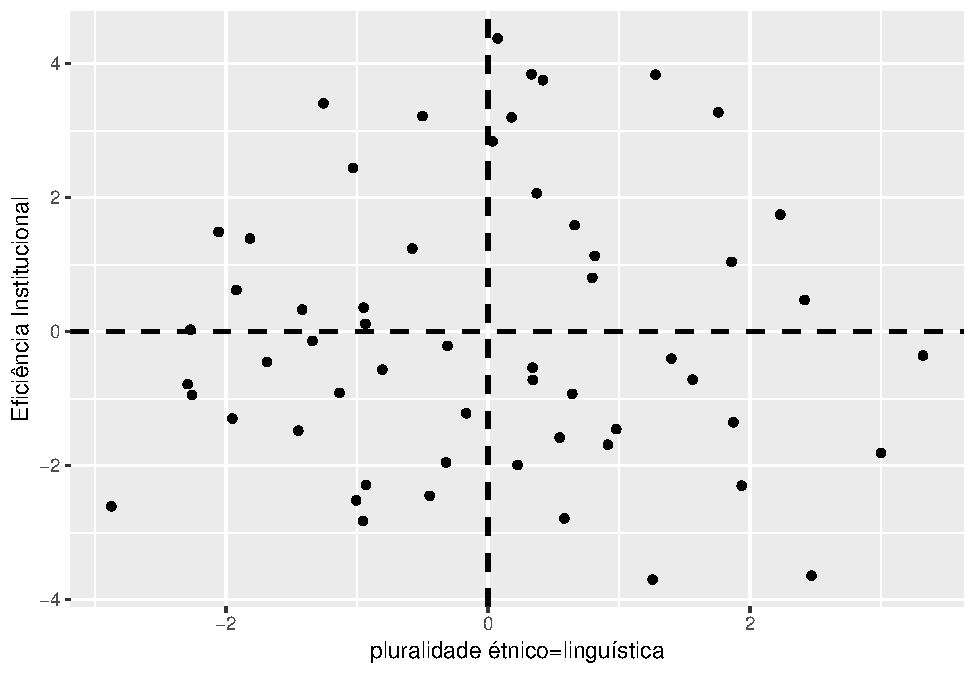
\includegraphics{Artigo_ad_files/figure-latex/unnamed-chunk-1-1.pdf}

\section*{References}\label{references}
\addcontentsline{toc}{section}{References}

\end{document}


